\documentclass[a4paper, 10pt]{book}
\usepackage[latin1]{inputenc}    % Accept european-encoded (latin1) characters.
\usepackage{a4wide}              % Wide paper
\usepackage[parfill]{parskip}		% skip a line instead of indenting new paragraphs
\usepackage{graphicx}   % For eps figures
\usepackage{epsfig}     % Alternative package
\usepackage{fancyhdr} 
\usepackage[hang,small,bf]{caption}
\usepackage{palatino}
\usepackage{amsmath}
\usepackage{amssymb}
\usepackage[vlined,linesnumbered,ruled]{algorithm2e}
\usepackage{color}
\usepackage{xcolor}
\usepackage{calc}

%% now change the chapter style
%% load up the quotchap package
\RequirePackage[avantgarde]{quotchap}

%% make the quotation appear next to the chapter number
\renewcommand\chapterheadstartvskip{\vspace*{-5\baselineskip}}

%% now change the section heading to have a line beneath it
%% load up the fancy title-style package
\RequirePackage[calcwidth]{titlesec}

\titleformat{\section}[hang]{\sffamily\bfseries}
{\Large\thesection}{12pt}{\Large}[{\titlerule[0.5pt]}]


\fancyhead[L]{\assignment }
\fancyhead[R]{\course \;- \instructor }
\renewcommand{\footrulewidth}{0.5pt} % Insert a line above the footer

%% make the odd pages have the section name on the top right
\fancyhead[RO]{\sffamily\bfseries \rightmark}
%% make the even pages have the chapter name on the top left
\fancyhead[LE]{\sffamily\bfseries \leftmark}

\newcommand{\problem}[1]{\subsection*{Problem #1}}

\newcommand{\answer}{\paragraph{Answer:}}

\newcommand{\proof}{\paragraph{Proof:}}

\newcommand{\qed}{\hfill \ensuremath{\Box}}

\newcommand{\red}[1]{\textcolor{red}{#1}}

\newcommand{\todo}{\textcolor{red}{TODO}{} }


\renewcommand{\chaptername}{}


\begin{document}

\author{Santa Zhang}
\title{Algorithms and Complexity Homework}
\maketitle

\tableofcontents

\chapter{Homework 1}

\problem{2.3-3}

Use mathematical induction to show that when $n$ is an exact power of 2, the solution of the recurrence

\begin{equation*}
T(n) = \left\{
  \begin{array}{ll}
    2         & \text{if $n=2$,}\\
    2T(n/2)+n & \text{if $n=2^k$, for $k>1$}
  \end{array}
\right.
\end{equation*}

is $T(n)=n\lg n$.

\proof

Assume $n = 2^k$, we perform mathematical induction on $k$. When $k =1$, we have $T(2^k) = T(2) = 2 = 2\times \lg 2$, the recurrence holds true.
If the recurrence is true for $ k \leq k_0$, then for $k = k_0 + 1$, we have:

\begin{eqnarray*}
T(2^{k_0 + 1}) &=& 2T\left(\frac{2^{k_0 + 1}}{2}\right) + 2^{k_0 + 1}\\
&=& 2T(2^{k_0}) + 2^{k_0 + 1}\\
&=& 2\times 2^{k_0} \times k_0 + 2^{k_0 + 1}\\
&=& 2^{k_0 + 1} \times (k_0 + 1),
\end{eqnarray*}

the solution is still true. So by mathematical induction, we have proved the recurrence.
\qed

\problem{2.3-6}

Observe that the \textbf{while} loop of lines 5-7 of the \textsc{Insertion-Sort} procedure below uses a linear search to scan (backward)
through the sorted subarray $A[i..j-1]$. Can we use a binary search instead to improve the overall worst-case running
time of insertion sort to $\Theta(n\lg n)$?

\begin{algorithm}[H]
\caption{\textsc{Insertion-Sort}}
\For{$j \leftarrow 2$ \KwTo $length[A]$}{
  $key \leftarrow A[j]$\\
  $\rhd$ Insert $A[j]$ into the sorted sequence $A[1..j-1]$.\\
  $j \leftarrow j - 1$\\
  \While {$i > 0$ and $A[i] > key$} {
    $A[i + 1] \leftarrow A[i]$ \\
    $i \leftarrow i -1 $
  }
  $A[i + 1] \leftarrow key$
}
\end{algorithm}


\answer

It is not possible. In each round of the \textsc{Insertion-Sort}, the algorithm first \textbf{finds the point to insert} and then \textbf{insert data},
each has cost of $\Theta(n)$. By using binary search, we could reduce the time for \textbf{finding the point to insert} to $\Theta(\lg n)$,
but it still has cost of $\Theta(n)$  to \textbf{insert data} in worst case. So the overall cost is still $n\times \Theta(n) = \Theta(n^2)$.
\qed

\problem{2-4 Inversions}

Let $A[1..n]$ be an array of $n$ distinct numbers. If $i<j$ and $A[i]>A[j]$, then the pair $(i,j)$ is called an \textbf{inversion} of $A$.

\begin{description}
\item[a. \hspace{9pt}] List the five inversions of the array $\langle2, 3, 8, 6, 1\rangle$.

\item[b. \hspace{9pt}] What array with elements from the set ${1, 2, ..., n}$ has the most inversions? How many does it have?

\item[c. \hspace{9pt}] What is the relationship between the running time of insertion sort and the number of inversions in the input array? Justify your answer.

\item[d. \hspace{9pt}] Give an algorithm that determines the number of inversions in an permutation on $n$ elements in $\Theta(n\lg n)$ worst-case time. (Hint: Modify merge sort.)
\end{description}

\answer

\begin{description}
\item[a. \hspace{9pt}] $(1, 5), (2, 5), (3, 5), (4, 5), (3, 4)$.

\item[b. \hspace{9pt}] The array $[n, n -1, n - 2, ..., 2, 1]$ has most inversions. It has ${{n}\choose{2}} = \frac{n(n - 1)}{2}$ inversions.

\item[c. \hspace{9pt}] The running time of insertion sort is \textbf{linear corelational} to the number of inversions in the input array.
This is true, because each time an element is moved, the number of inversion pairs is reduced by one. So the number of move action is equal to
the number of inversion pairs, and since move action requires constant time, we know the conlusion is true.

\item[d. \hspace{9pt}] Sorted arrays have 0 inversion pairs. Given 2 sorted array $A=(a_0, a_1, ..., a_m)$ and $B = (b_0, b_1, ..., b_n)$,
and let $\overline{AB} = (a_0, a_1, ..., a_m, b_0, b_1, ..., b_n)$. The number of inversions in $\overline{AB}$ could be caculated by the following method:

For any $a_i$ in $\overline{AB}$, suppose we could find such an $j$ that $b_j < a_i < b_{j + 1}$, then we know that there are $j$ numbers in $\overline{AB}$
which are smaller than $a_i$, introducing $j$ inversion pairs. Otherwise we cannot find a proper $j$, we know that there is no inversion pair for $a_i$.
For any $b_j$ in $\overline{AB}$ we have similar results.

So we could write the following algorithm for counting inversion pairs, similar to \textsc{Merge-Sort}, it has a complexity of $\Theta(n\lg n)$:

\begin{algorithm}[H]
\caption{\textsc{Inversion-Pair}}
\SetKwInOut{Input}{input}
\SetKwInOut{Output}{output}
\Input{$A$: an array, $p$ \& $q$: index for array $A$}
\Output{The number of inversion pairs in $A[p...q]$, inclusive}
\If{$ p\geq q$}{
  \KwRet 0\tcp*[r]{at most 1 item, there is no inversion}
}
\Else{
  \tcp{$S$: number of inversion pairs}
  $S \leftarrow  $ \textsc{Inversion-Pair}$(A, p, k)$ + \textsc{Inversion-Pair}$(A, k + 1, q)$\\
  $i \leftarrow 1$, $j \leftarrow 1, k \leftarrow \lfloor\frac{p + q}{2}\rfloor$\\
  $L \leftarrow A[p...k], R \leftarrow A[k + 1...q]$\\
  clear array $A$\\
  \While{$i < length(L)$ and $j < length(R)$}{
    \If{$L_i < R_j$}{
      append $L_i$ to $A$\\
      $i \leftarrow i + 1$\\
    }
    \ElseIf {$L_i > R_j$}{
      append $R_j$ to $A$\\
      $S \leftarrow S + (length(L) - i + 1)$\\
      $j \leftarrow j + 1$\\
    }
    \Else {
      \tcp{$L_i = R_j$}
      append $L_i$ and $R_j$ to $A$\\
      $i \leftarrow i + 1$\\
      $j \leftarrow j + 1$\\
      }
  }
  $S \leftarrow S +  length(R) \times (length(L) - i + 1)$\\
  append the rest of $L$ to $A$\\
  append the rest of $R$ to $A$\\
  \KwRet $S$
}
\end{algorithm}

\end{description}
\qed


\problem{3.2-3} Prove equation (3.18). Also prove that $n! = \omega(2^n)$ and $n! = o(n^n)$.

\begin{equation}
\lg(n!) = \Theta(n\lg n)
\tag{3.18}
\end{equation}

\proof

With Stirling's equation:

\begin{eqnarray*}
\lg (n!) &=& \lg\left(\sqrt{2\pi n}\left(\frac{n}{e}\right)^n\left(1 + \Theta\left(\frac{1}{n}\right)\right)\right)\\
&=& \frac{1}{2}\lg n + n(\lg n - \lg e) + \Theta(1)\\
&=& n \lg n + \Theta(n)\\
&=& \Theta(n \lg n).
\end{eqnarray*}

Since $\lg 2^n = n = o(n\lg n)$, we have $n ! = \omega(2^n)$.

And by Stirling's equation:

\begin{eqnarray*}
n! &=& \sqrt{2\pi n}\left(\frac{n}{e}\right)^n\left(1 + \Theta\left(\frac{1}{n}\right)\right)\\
&<& n^n \times \frac{\sqrt{2\pi n}}{e^n} \times 2\\
&=& n^n \times \omega(1),
\end{eqnarray*}

So we have $n! = o(n^n)$.
\qed

\problem{3-3 Ordering by asymptotic growth rates}

\begin{description}
\item[a. \hspace{9pt}] Rank the following functions by order of growth; that is, find an arrangement $g_1, g_2, ..., g_{30}$ of the functions satisfying
$g_1 = \Omega(g_2), g_2 = \Omega(g_3), ..., g_{29} = \Omega(g_{30})$. Partition your list info equivalence classes such that $f(n)$ and $g(n)$
are in the same class if and only if $f(n) = \Theta(g(n))$.

\begin{equation*}
\begin{array}{cccccc}
\lg(\lg^*n)                 & 2^{\lg^*n}          & \left(\sqrt 2\right)^{\lg n}  & n^2           & n!        & (\lg n)!\\
\left(\frac{3}{2}\right)^n  & n^3                 & \lg^2n                        & \lg(n!)       & 2^{2^n}   & n^{\frac{1}{\lg n}}\\
\ln\ln n                    & lg^*n               & n \cdot 2^n                   & n^{\lg\lg n}  & \ln n     & 1\\
2^{\lg n}                   & (\lg n)^{\lg n}     & e^n                           & 4^{\lg n}     & (n+1)!    &  \sqrt{\lg n}\\
\lg^*(\lg n)                & 2^{\sqrt{2 \lg n}}  & n                             & 2^n           & n\lg n    & 2^{2^{n+1}}
\end{array}
\end{equation*}

\item[b. \hspace{9pt}] Give an example of a single nonnegative function $f(n)$ such that for all functions $g_i(n)$ in part (a), $f(n)$ is neither $O(g_i(n))$
nor $\Omega(g_i(n))$.
\end{description}

\answer

\begin{description}

\item[a. \hspace{9pt}] First of all, we have 
$$n^{\frac{1}{\lg n}} = n^{\log_n{2}} = 2,$$

which means $n^{\frac{1}{\lg n}} = \Theta(1).$ Constant numbers has zero growth, so they are in the lowest class.

Let $f(x) = 2^x$, then we have $\log^*{\left(f^{(t)}(1)\right)} = t$ and $\lg\left(f^{(t)}(1)\right) = \lg\left(2^{f^{(t-1)}(1)}\right) = f^{(t-1)}(1)$. Now assume $n = f^{(t)}(1)$, we have:

\begin{eqnarray*}
\lg\left(\lg^*n\right) &=& \lg\left(\lg^*\left(f^{(t)}(1)\right)\right) = \lg t\\
\lg^*\left(\lg n\right) &=& \lg^*\left(\lg \left(f^{(t)}(1)\right)\right) = \lg^*\left(f^{(t-1)}(1)\right) = t-1\\
\lg^*(n) &=& \lg^*\left(f^{(t)}(1)\right) = t\\
2^{\lg^*\left(\lg n\right)} &=& 2^t\\
\ln\ln n &=& \ln \left(\ln \left(f^{(t)}(1)\right)\right) = \Theta\left(f^{(t - 2)}(1)\right).
\end{eqnarray*}

Since $\lg t < t - 1 \sim t < 2^t <\Theta\left(f^{(t - 2)}(1)\right)$ when $t$ is big enough, we know that:

\begin{equation}
\lg\left(\lg^*n\right) < \lg^*\left(\lg n\right) \sim \lg^*n < 2^{\lg^*n} < \ln \ln n.
\end{equation}

Now assume $n = 2^t$, we have:

\begin{eqnarray*}
\ln\ln n &=& \ln \ln \left(2^t\right) = \Theta\left(\lg t\right)\\
\sqrt{\lg n} &=& \sqrt{t}\\
\ln n &=& \Theta(t)\\
\lg^2{n} &=& \left(\lg2^t\right)^2 =  t^2 = 2^{2\lg t}\\
2^{\sqrt{2\lg n}} &=& 2^{\sqrt{2t}}\\
\left(\sqrt{2}\right)^{\lg n} &=& 2^{\frac{t}{2}}\\
n &=& 2^t.
\end{eqnarray*}

From those equations we have:

\begin{equation}
\ln \ln n  < \sqrt{\lg n} < \ln n < \lg^2 n < 2^{\sqrt{2\lg n}} < \left(\sqrt{2}\right)^{\lg n}  < n.
\end{equation}

And it is easy to sort those functions:

\begin{equation}
n = 2^{\lg n} < n \lg n \sim \lg\left(n !\right) < n^2 = 4^{\lg n} < n^3,
\end{equation}

with the fact that:

\begin{eqnarray*}
\lg (n!) &=& \lg \left(\sqrt{2\pi n} \left(\frac{n}{e}\right)^n\left(1 + \Theta\left(\frac{1}{n}\right)\right)\right)\\
&=& \frac{1}{2}\ln n + n(\ln n - 1) + \Theta(1)\\
&=& \Theta(n \ln n).
\end{eqnarray*}

It is trivial to prove that $8^t < t!$. Replace $t$ with $\lg n$, we have

$$8^{\lg n} = n^3 < (\lg n)!.$$

To compare $(\lg n)!$ and $n^{\lg \lg n}$,  we have:

\begin{eqnarray*}
\lg \left((\lg n)! \right) &=& \frac{1}{2} \ln \lg n + \lg n \times (\ln \lg n - 1) + \Theta(1)\\
&=& \frac{1}{\lg e}\times \lg n \times \lg \lg n + \Theta(\lg n)\\
\lg \left(n^{\lg \lg n}\right) &=& \lg n \times \lg \lg n,
\end{eqnarray*}

which means:

$$(\lg n)! < n^{\lg \lg n}.$$

To compare $ n^{\lg \lg n}$ and $(\lg n)^{\lg n}$, we have:

\begin{eqnarray*}
\lg \left(n ^ {\lg \lg n}\right) &=& \lg n \times \lg \lg n\\
\lg \left(\left(\lg n\right)^{\lg n}\right) &=& \lg n \times \lg \lg n,
\end{eqnarray*}

which means:

$$ n^{\lg \lg n}  = (\lg n)^{\lg n}.$$

To compare $(\lg n)^{\lg n}$ and $\left(\frac{3}{2}\right)^n$, we have:

\begin{eqnarray*}
\lg \left( \frac{3}{2}\right)^n &=& n\times \lg \left(\frac{3}{2}\right) > \lg^2 n > \lg n\times \lg \lg n = \lg \left(\left(\lg n\right)^{\lg n}\right),
\end{eqnarray*}

which means:

$$ (\lg n)^{\lg n} < \left(\frac{3}{2}\right) ^ n.$$

And it is easy to sort these functions:

$$ \left(\frac{3}{2}\right)^n < 2^n < n \cdot 2^n < e^n < ( n^n  <) n!  < (n + 1)!.$$

To compare $(n + 1)!$ and $2^{2^n}$, we have:

\begin{eqnarray*}
\lg (n + 1)! &=& \Theta(n \lg n)\\
\lg \left(2^{2^n}\right) &=& 2^n,
\end{eqnarray*}

which means $(n + 1)! < 2^{2^n}$.

And finally we have $2^{2^n} < 2^{2^{n + 1}}$.

Now we could conclude the problem:

\begin{eqnarray*}
1 \sim n^{\frac{1}{\lg n}} < \lg \left(\lg^*n\right) < \lg^*\left(\lg n\right) \sim \lg^* n < 2^{\lg^* n} < \ln\ln n < \sqrt{\lg n} < \ln n < \lg^2 n\\
< 2^{\sqrt{2\lg n}} < \left(\sqrt 2\right) ^ {\lg n} < n = 2^{\lg n}  < n\lg n \sim \lg \left(n!\right) < n^2 = 4^{\lg n}< n^3  < (\lg n)!\\
< n^{\lg \lg n} = \left(\lg n \right)^{\lg n} < \left(\frac{3}{2}\right)^n < 2^n < n\cdot 2^n < e^n < n! < (n + 1)! < 2^{2^n} < 2^{2^{n + 1}}
\end{eqnarray*}

\item[b. \hspace{9pt}] This function is a solution:

$$(1 + \sin(n)) \times 3^{3^n}.$$

\end{description}
\qed




\chapter{Homework 2}

\problem{4.1-2}

We saw that the solution of $T(n) = 2T(\lfloor\frac{n}{2}\rfloor) + n$ is $O(n\lg n)$. Show that the slution of this recurrence is also $\Omega(n \lg n)$.
Concolude that the solution is $\Theta(n \lg n)$.

\answer

Assume that $2^p \leq n < 2^{p-1}$, we have:

\begin{eqnarray*}
T(n) &=& 2T\left(\left\lfloor\frac{n}{2}\right\rfloor\right) + n\\
&=& 4T\left(\left\lfloor\frac{n}{4}\right\rfloor\right) + 2\times\left\lfloor\frac{n}{2}\right\rfloor + n\\
&\geq& 4T\left(\left\lfloor\frac{n}{4}\right\rfloor\right) + 2\times\left\lfloor\frac{2^p}{2}\right\rfloor + n\\
&=& 4T\left(\left\lfloor\frac{n}{4}\right\rfloor\right) + 2^p + n\\
&=& \cdots\\
&\geq& 2^k T\left(\left\lfloor\frac{n}{2^k}\right\rfloor\right) + 2^p \times (k - 1) + n\\
&=& 2^{k + 1} T\left(\left\lfloor\frac{n}{2^{k + 1}}\right\rfloor\right) + 2^k\times\left\lfloor\frac{n}{2^k}\right\rfloor  +2^p \times (k - 1) + n\\
&\geq& 2^{k + 1} T\left(\left\lfloor\frac{n}{2^{k + 1}}\right\rfloor\right) + 2^k\times\left\lfloor\frac{2^p}{2^k}\right\rfloor  +2^p \times (k - 1) + n\\
&=& 2^{k + 1} T\left(\left\lfloor\frac{n}{2^{k + 1}}\right\rfloor\right)  +2^p \times k + n\\
&=& \cdots\\
&\geq& 2^p T\left(\left\lfloor\frac{n}{2^p}\right\rfloor\right) + 2^p \times (p - 1) + n\\
&=& 2^p T(1) + 2^p \times (p - 1) + n\\
&>& 2n T(1) + 2n \lg n + n\\
&=& \Theta(n\lg n)
\end{eqnarray*}

Since $T(n)\geq \Theta(n\lg n)$, we have $T(n) = \Omega(n \lg n)$. Now we know that $T(n) = \Omega(n\lg n)$ and $T(n) = O(n \lg n)$, so $T(n) = \Theta(n\lg n)$.
\qed

\problem{4.2-1}

Use a recursion tree to determine a good asymptotic upper bound on the recurrence $T(n) = 3T(\lfloor\frac{n}{2}\rfloor) + n$. Use the substitution method to verify your answer.

\answer

Assume the answer is $T(n) = c\times n^{\lg3} - bn, 0 < b \leq 2, c > 0$. For $n > 3$, we have:

\begin{eqnarray*}
T(n) &=& 3T\left(\left\lfloor\frac{n}{2}\right\rfloor\right) + n\\
&=& 3c\times\left(\left\lfloor\frac{n}{2}\right\rfloor\right)^{\lg3} - 3b\left\lfloor \frac{n}{2}\right\rfloor + n\\
&\leq& 3c\times\left(\left\lfloor\frac{n}{2}\right\rfloor\right)^{\lg3} - 3b\times \frac{n -1}{2} + n\\
&=& 3c\times\left(\left\lfloor\frac{n}{2}\right\rfloor\right)^{\lg3} - \left(\frac{3b}{2} - 1\right)n + \frac{3b}{2}\\
&\leq& 3c \times \left(\frac{n}{2}\right)^{\lg3} - \left(\frac{3b}{2}- 1\right)n + n \text{\hspace{9pt}(note that $0 < b \leq 2$ and $n > 3$)}\\
&=& c\times n^{\lg3} - \left(\frac{3b}{2} - 2\right)n
\end{eqnarray*}

In order to make the following equation true, we only have to choose $c = 1, b = 2$:

$$c\times n^{\lg3} - bn \leq c\times n^{\lg3} - \left(\frac{3b}{2} - 2\right)n.$$

So now we have proved $T(n) = \Theta(n^{\lg 3}).$
\qed

\problem{4.3-1}

Use the master method to give tight asymptotic bounds for the following recurrences.

\begin{description}
\item[a. \hspace{9pt}] $T(n) = 4T(\lfloor\frac{n}{2}\rfloor) + n$.
\item[b. \hspace{9pt}] $T(n) = 4T(\lfloor\frac{n}{2}\rfloor) + n ^ 2$.
\item[c. \hspace{9pt}] $T(n) = 4T(\lfloor\frac{n}{2}\rfloor) + n ^ 3$.
\end{description}

\answer

\begin{description}
\item[a.\hspace{9pt}] $T(n) = \Theta(n^2)$.
\item[b.\hspace{9pt}] $T(n) = \Theta(n^2\lg n)$.
\item[c.\hspace{9pt}] $T(n) = \Theta(n^3)$.
\end{description}
\qed

\problem{5.1-3}

Suppose that you want to output 0 with probability $\frac{1}{2}$ and 1 with probability $\frac{1}{2}$. At your disposal is a procedure \textsc{Biased-Random}, that outputs
either 0 or 1. It outputs 1 with some probability $p$ and 0 with probability $1-p$, where $0 < p < 1$, but you do not know that $p$ is. Give an algorithm that uses
\textsc{Biased-Random} as a subroutine, and returns an unbiased answer, returning 0 with probility $\frac{1}{2}$ and 1 with probability $\frac{1}{2}$. What is the expected
running time of your algorithm as a function of $p$?

\answer

If we call \textsc{Biased-Random} twice, we could get one of $00, 01, 10, 11$. The probability of $01$ and $10$ are both $p(1-p)$, if we consider $01$ as $1$ and $10$ as $0$,
then we have could generate $1$ and $0$ with equal probability of $\frac{1}{2}$. And if we got $00$ or $11$, just keep calling \textsc{Biased-Random} until we reached 
$10$ or $01$. So we could use the following procedure:

\begin{algorithm}[H]
\caption{\textsc{Fairly-Random}}
\While{forever} {
  $a \leftarrow$ \textsc{Biased-Random}\\
  $b \leftarrow$ \textsc{Biased-Random}\\
  \If{$a = 0$ and $b = 1$}{
    \Return 1
  }\ElseIf {$a = 1$ and $b = 0$} {
    \Return 0
  }
}
\end{algorithm}

Now we could analyze the running time of the algorithm. On each round of the \textbf{while} loop, we have a probabily of $2p(1-p)$ to \textbf{return}. So by the property of
geometry distribution, the \textbf{while} loop will be executed $\frac{1}{2p(1-p)}$ times, which means the running time of the procedure is $\Theta\left(\frac{1}{2p(1-p)}\right)$.
\qed

\problem{5.3-4}

Professor Armstrong suggests the following procedure for generating a uniform random permutation:

\begin{algorithm}[H]
\caption{\textsc{Permute-By-Cycle}$(A)$}
$n \leftarrow length[A]$\\
$offset \leftarrow$\textsc{Random}$(1, n)$\\
\For{$i \leftarrow 1$ \KwTo $n$}{
  $dest \leftarrow i + offset$\\
  \If {$dest > n$} {
    $dest \leftarrow dest - n$
  }
  $B[dest] \leftarrow A[i]$
}
\Return $B$
\end{algorithm}

Show taht each element $A[i]$ has a $\frac{1}{n}$ probability of winding up in any particular position in $B$. Then show that Professor Armstrong is mistaken by showing
that the resulting permutation is not uniformly random.

\answer

The value of $offset$ is uniformly distributed in $[1, n]$, that means we have 
$$P(offset = k| k\in [1, n]) = \frac{1}{n}.$$

Let the indicator $X_{i, j}$ be the probability of ``$A[i]$ end up in $B[j]$''. We have:

\begin{eqnarray*}
X_{i, j} &=& P\left(offset = (j - i + n)\mod n\right)\\
&=& P(offset = k| k\in [1, n])\\
&=& \frac{1}{n}.
\end{eqnarray*}

Now we prove that the procedure cannot generate uniform permutation. Consider that case where $n>2$, we observe the permutation result on $A[1]$ and $A[2]$.
If the procedure generates uniform permutation, then there is $\frac{1}{2}$ probability that $A[2]$ ends up ahead of $A[1]$, in array $B$. But
 $A[2]$ ends up ahead of $A[1]$ only happens when $offset = n - 1$. The probability of $offset = n - 1$ is $\frac{1}{n} \neq \frac{1}{2}$. So the procedure
cannot generate uniform permutation.
\qed

\problem{5.4-2}

Suppose that balls are tossed into $b$ bins. Each toss is independent, and each ball is equally likely to end up in any bin. What is the expected number of ball tosses
before at least one of the bins contains two balls?

\answer

Let us consider the situation where in the first $k$ tosses, every bin contains at most $1$ ball. In this case, the first $k$ numbers will be a permutation on $b$.
And the whole sample space is $b^k$, since each time we could choose any one of the $b$ bins. So the probability that ``in the first $k - 1$ tosses, every bin contains
at most $1$ ball'' is $\frac{P^{k- 1}_b}{b^{k - 1}} = \frac{b!/(b-k + 1)!}{b^{k - 1}} = \frac{b!}{b^{k - 1}(b-k + 1)!}$. Thus we know that the probability that
``exactly in the $k$th toss, the target bin contains 2 balls for the first time'' is $\frac{k - 1}{b}\times\frac{b!}{b^{k - 1}(b - k + 1)!}$. So finally we have the expected number of ball tosses:

$$\sum_{k = 1}^{b + 1}\left(k\times\frac{k - 1}{b} \times \frac{b!}{b^{k - 1}(b - k + 1)!}\right) = \sum_{k = 1}^{b + 1} \left(\frac{k(k - 1)b!}{b^k(b - k + 1)!}\right).$$

On the other hand, this problem is similar to the ``Birthday paradox'', so by the same reasoning we know that the answer should be in the range $\Theta(\sqrt{b})$.
\qed




\chapter{Homework 3}

\problem{6.3-2}
Why do we want the loop index $i$ in line 2 of \textsc{Build-Max-Heap} to decrease from $\left\lfloor \frac{length[A]}{2}\right\rfloor$ to $1$ rather than increase from $1$
to $\left\lfloor \frac{length[A]}{2}\right\rfloor$?

\begin{algorithm}[H]
\caption{\textsc{Build-Max-Heap}$(A)$}
$heap$-$size[A]\leftarrow length[A]$\\
\For{$i \leftarrow \left\lfloor\frac{length[A]}{2}\right\rfloor$ \textnormal{\textbf{downto}} $1$} {
  \textsc{Max-Heapify}$(A, i)$
}
\end{algorithm}

\answer

This is because we must make sure that the smaller subtrees are changed to heaps first, so that the algorithm could build bigger subtrees correctly. If we increase the index $i$ from $1$ to
$\left\lfloor\frac{length[A]}{2}\right\rfloor$, the heap property cannot be correctly preserved.
\qed

\problem{6.5-7}
The operation \textsc{Heap-Delete}$(A, i)$ deletes the item in node $i$ from heap $A$. Give an implementation of \textsc{Heap-Delete} that runs in $O(\lg n)$ time for an $n$-element
max-heap.

\answer

The implementation is given below. Since both \textsc{Max-Heapify}$(A, i)$ and \textsc{Heap-Increase-Key}$(A, i, key)$ runs in $O(\lg n)$ time, \textsc{Heap-Delete}$(A, i)$ also runs in $O(\lg n)$.

\begin{algorithm}[H]
\caption{\textsc{Heap-Delete}$(A, i)$}
$n \leftarrow heap$-$size[A]$\\
$heap$-$size[A] \leftarrow heap$-$size[A] - 1$\\
\If{$A[i] < A[n]$}{
  \textsc{Heap-Increase-Key}$(A, i, A[n])$\\
}\Else{
  $A[i] \leftarrow A[n]$\\
  \textsc{Max-Heapify}$(A, i)$\\
}
\end{algorithm}
\qed

\problem{7-1 Hoare partition correctness}
The version of \textsc{Partition} given in this chapter is not the original partitioning algorithm. Here is the original parition algorithm, which is due to T.Hoare:

\begin{algorithm}[H]
\caption{\textsc{Hoare-Partition}(A, p, r)}
$x \leftarrow A[p]$\\
$i \leftarrow p - 1$\\
$j \leftarrow r + 1$\\
\While{$true$}{
  \Repeat{$A[j] \leq x$}{
    $j \leftarrow j - 1$\\
  }
  \Repeat{$A[i] \geq x$}{
    $i \leftarrow i + 1$\\
  }
  \If{$i < j$}{
    exchange $A[i] \leftrightarrow A[j]$
  }\Else{
    \Return $j$
  }
}
\end{algorithm}

\begin{description}
\item[a. \hspace{9pt}] Demonstrate the operation of \textsc{Hoare-Partition} on the array $A=\langle13, 19, 9, 5, 12, 8, 7, 4, 11,\\ 2, 6, 21\rangle$, showing the values of
the array and auxiliary values after each iteration of the \textbf{while} loop in lines $4-11$.\\

\end{description}
The next three questions ask you to give a careful argument that the procedure \textsc{Hoare-Partition} is correct. Prove the following:

\begin{description}
\item[b. \hspace{9pt}] The indices $i$ and $j$ are such that we never access an element of $A$ outside the subarray $A[p\ldots r]$.

\item[c. \hspace{9pt}] When \textsc{Hoare-Partition} terminates, it returns a value $j$ such that $p\leq j < r$.

\item[d. \hspace{9pt}] Every element of $A[p\ldots j]$ is less than or equal to every element of $A[j + 1\ldots r]$ when \textsc{Hoare-Partition} terminates.
\end{description}

The \textsc{Partition} procedure shown below separates the pivot value (originally in $A[r]$) from the two partitions it forms. The \textsc{Hoare-Partition} procedure,
on the other hand, always places the pivot value (originally in $A[p]$) into one of the two paritions $A[p\ldots j]$ and $A[j + 1\ldots r]$. Since $p\leq j < r$, this
split is always nontrivial.

\begin{algorithm}[H]
\caption{\textsc{Partition}(A, p, r)}
$x\leftarrow A[r]$\\
$i \leftarrow p - 1$\\
\For{$j \leftarrow p$ \KwTo $r-1$}{
  \If{$A[j] \leq x$} {
    $i \leftarrow i + 1$\\
    exchange $A[i] \leftrightarrow A[j]$\\
  }
}
exchange $A[i + 1]\leftrightarrow A[r]$\\
\Return {$i + 1$}
\end{algorithm}

\begin{description}
\item[e. \hspace{9pt}] Rewrite the \textsc{Quicksort} procedure to use \textsc{Hoare-Partition}.
\end{description}

\answer

\begin{description}
\item[a. \hspace{9pt}] The iteration is shown in the following table:

\begin{center}
\begin{tabular}{|c|c|c|c|}
\hline
Loop No. & $A$ & $i$ & $j$\\\hline
1 & $\langle 6, 19, 9, 5, 12, 8, 7, 4, 11, 2, 13, 21\rangle$ & 1 & 11\\\hline
2 & $\langle 6, 2, 9, 5, 12, 8, 7, 4, 11, 19, 13, 21\rangle$ & 2 & 10\\\hline
3 & $\langle 6, 2, 9, 5, 12, 8, 7, 4, 11, 19, 13, 21\rangle$ & 10 & 9\\\hline
\end{tabular}
\end{center}

\item[b. \hspace{9pt}] First of all, $j$ was given initial value $r + 1$, and it is decreased before the access of $A[j]$, so $j\leq r$ when $j$ is used as an index to $A$.
Similarly we have $i \geq p$.

Suppose that when the procedure \textbf{return}s, there is a $k$ such that $j < k < i$. Since the \textbf{repeat} statement of lines $5 \sim 7$ halts only when $A[j] \leq x$, 
we know that $A[k] > x$. Similarly, the \textbf{repeat} statement of lines $8 \sim 10$ halts only when $A[j] \geq x$, which requires $A[k] < x$. From this contradiction we knows
that the $k$ does not exist, which means $j \geq i - 1$.

On each round of the \textbf{while} loop, line 6 and line 9 are both executed at least once. If the \textbf{while} loop is executed more than once, we have $j \leq r - 1$ and
$i \geq p + 1$. With the fact that $j \geq i -1$, it is trivial to prove that  $p \leq i \leq r$ and $p \leq j \leq r$.


Now we consider the case when the \textbf{while} loop is executed only once. The \textbf{repeat} statement of lines $5 \sim 7$ halts when $A[j] \leq x$. With the fact that $A[p] = x$,
we have $j \geq p$. And the \textbf{repeat} statement of lines $8 \sim 10$ will halt with $i = p$. Now we have proved that under all cases, $p \leq i \leq r$ and $p \leq j \leq r$, 
so we never access an element of $A$ outside $A[p\ldots r]$.

\item[c. \hspace{9pt}] The original question should add another requirement that $p < r$. We have already proved that $p \leq j \leq r$. Suppose the procedure returned $j = r$, then
we know that the \textbf{while} loop is executed only once (in each \textbf{while} loop, $j$ is decreased at least by 1). And we know that on the first round of the \textbf{while}
loop, the \textbf{repeat} statement of lines $8 \sim 10$ will halt with $i = p$. The \textbf{return} statement will be reached only when $i \geq j$, that is, $p \geq r $. Now we have
a contradiction here, which means $j \neq r$, so the procedure returns $p \leq j < r$.

\item[d. \hspace{9pt}] We prove the invariant that ``after line 10, every element in $A[p \ldots i - 1]$ is less than or equal to $x$, and every element in $A[j + 1 \ldots r]$ is greater than
or equal to $x$''.

Before the first round of the \textbf{while} loop, this invariant is true, since there is no element in the subarrays. Suppose the invariant is true before the $k$th round, then in the $k$th
round, the \textbf{repeat} statement in lines $5 \sim 7$ decrease $j$ until $A[j] \leq x$, so it is still true that any element in $A[j + 1 \ldots r]$ is greater than or equal to $x$.
Similarly we know that any element in $A[p \ldots i - 1]$ is less than or equal to $x$. Lines $11\sim 14$ does not change the value of $i$ and $j$, so $i$ and $j$ remains unchanged until
the $(k + 1)$th loop. By mathematical induction we know that the invariant is true.

The procedure returns only when $i \geq j$, and we have proved $j \geq i - 1$ in question (c), so we have either $i = j$ or $i = j + 1$. If $i = j$, since $A[i] \geq x$ and $A[j] \leq x$, 
we have $A[i] = A[j] = x$, so every element in $A[p \ldots j]$ is less than or equal to $x$, and every element in $A[j + 1 \ldots r]$ is greater than or equal to $x$. If $i = j + 1$,
we have the same conclusion. Thus the statement of question (d) is proved.

\item[e. \hspace{9pt}] The algoritm is given below.

\end{description}
\begin{algorithm}[H]
\caption{\textsc{Hoare-Quicksort}(A, p, r)}
\If{$p \leq r$}{
  \Return
}\Else{
  $j \leftarrow$\textsc{Hoare-Partition}$(A, p, r)$\\
  \textsc{Hoare-Quicksort}$(A, p, j)$\\
  \textsc{Hoare-Quicksort}$(A, j + 1, r)$
}
\end{algorithm}
\qed

\problem{7-3 Stooge sort}
Professors Howard, Fine, and Howard have proposed the following ``elegant'' sorting algorithm:

\begin{algorithm}[H]
\caption{\textsc{Stooge-Sort}$(A, i, j)$}
\If{$A[i] > A[j]$}{
  exchange $A[i] \leftrightarrow A[j]$\\
}
\If{$i + 1 \geq j$}{
  \Return
}
$k\leftarrow \left\lfloor\frac{j - i + 1}{3}\right\rfloor$\tcp*[r]{Round down.}
\textsc{Stooge-Sort}$(A, i, j - k)$\tcp*[r]{First two-thirds.}
\textsc{Stooge-Sort}$(A, i +k, j)$\tcp*[r]{Last two-thirds.}
\textsc{Stooge-Sort}$(A, i, j - k)$\tcp*[r]{First two-thrids again.}
\end{algorithm}

\begin{description}
\item[a. \hspace{9pt}] Argue that, if $n = length[A]$, then \textsc{Stooge-Sort}$(A, 1, length[A])$ correctly sorts the input array $A[1\ldots n]$.

\item[b. \hspace{9pt}] Give a recurrence for the worst-case running time of \textsc{Stooge-Sort} and a tight asymptotic ($\Theta$-notation) bound on the worst-case
running time.

\item[c. \hspace{9pt}] Compare the worst-case running time of \textsc{Stooge-Sort} with that of insert sort, merge sort, heapsort, and quicksort. Do the professors
deserve tenure?
\end{description}

\answer

\begin{description}
\item[a. \hspace{9pt}]

It is trivial to check that the algorithm is correct for $n = 1, 2, 3$. Suppose the algorithm is correct for $n \leq n_0, (n_0 \geq 3)$, now we prove that it is still correct for $n = n_0 + 1$.

We know that $k \geq 1$, so $A[i\ldots j - k]$ has less than $(n_0 + 1)$ elements. Since the algorithm is correct for $n \leq n_0$, $A[i \ldots j - k]$ is correctly sorted.
Suppose there is an element in $A[i \ldots j - k]$ that is larger than an element $x$ in $A[j - k + 1 \ldots j]$. Since $A[i \ldots j - k]$ is correctly sorted in line $8$, we know that 
$A[j - k]  > x$. Also, since $A[j -k + 1\ldots j]$ is correctly sorted in line $7$, we know that $A[j - k + 1] \leq x$. This leads to $A[j -k + 1] < A[j - k]$, however, $A[j - k + 1]$
and $A[j - k]$ should have been sorted in line $7$, this is a contradiciton. So we know that for $n = n_0 + 1$,  every element in $A[i \ldots j - k]$ is less than or equal to
$A[j -k +1 \ldots j]$, and both subarrays are correctly sorted, so the whole array $A$ is sorted. By mathematical induction, we have proved that the algorithm is correct for all $n$.

\item[b. \hspace{9pt}] The running time recurrence is

$$T(n) = 3 T\left(\frac{2n}{3}\right) + \Theta(1).$$

By Master Theorem, we have

$$T(n) = \Theta\left(n^{\log_{\frac{3}{2}}3}\right) \sim \Theta(n^{2.71}).$$

\item[c. \hspace{9pt}] The worst running time of \textsc{Insert-Sort} and \textsc{Quick-Sort} are both $\Theta(n^2)$, that of \textsc{Merge-sort} and \textsc{Heap-Sort}
are both $\Theta(n\lg n)$. Any of them has a much better running time than $\Theta(n^{2.71})$, so \textsc{Stooge-Sort} is not a very good sorting algorithm.

\end{description}
\qed




\chapter{Homework 4}
\problem{8.2-4}
Describe an algorithm that, given $n$ intergers in the range $0$ to $k$, preprocesses its input and then answers any query about how many of the $n$ integers fall into a range
$[a\ldots b]$ in $O(1)$ time. Your algorithm should use $\Theta(n + k)$ preprocessing time.
\answer

The algorithm is given below. The \textsc{Preprocess} returns an array, which will be used by \textsc{Count-Interval}.

\begin{algorithm}[H]
\caption{\textsc{Preprocess}$(A, n, k)$}
Create array $C$ with size $k + 1$, index starts at $0$\\
\For{$i = 0$ to $k$}{
  $C[i] \leftarrow 0$
}
\For{$i = 1$ to $n$}{
  $C[A[i]] \leftarrow C[A[i]] + 1$
}
\tcp{Now $C[j]$ contains number of elements with value $j$}
\For{$i = 1$ to $k$}{
  $C[A[i]] \leftarrow C[A[i]] + C[A[i - 1]]$
}
\tcp{Now $C[j]$ contains number of elements in the range $[0, j]$}
\Return $C$
\end{algorithm}

\begin{algorithm}[H]
\caption{\textsc{Count-Interval}$(C, a, b)$}
\tcp{Array $C$ is returned by \textsc{Preprocess}$(A, n)$}
\If{$a \neq 0$}{
  \Return $C[b] - C[a - 1]$
}\Else{
  \Return $C[b]$
}
\end{algorithm}
\qed


\problem{8-4}
Suppose that you are given $n$ red and $n$ blue water jugs, all of different shapes and sizes. All red jugs hold different amounts of water, as do the blue ones. Moreover,
for every red jug, there is a blue jug that holds the same amount of water, and vice versa.

It is your task to find a grouping of the jugs into pairs of red and blue jugs that holds the same amount of water. To do so, you may perform the following operation:
pick a pair of jugs in which one is red and one is blue, fill the red jug with water, and then pour the water into the blue jug. This operation will tell you whether the red or
blue jug can hold more water, or if they are of the same volume. Assume that such a comparison takes one time unit. Your goal is to find an algorithm that makes a minimum number of
comparisons to determine the grouping. Remember that you may not directly compare two red jugs or two blue jugs.

\begin{description}
\item[a. \hspace{9pt}] Describe a deterministic algorithm that uses $\Theta(n^2)$ comparisons to group the jugs into pairs.


\item[b. \hspace{9pt}] Prove a lower bound of $\Omega(n \lg n)$ for the number of comparisons an algorithm solving this problem must make.

\item[c. \hspace{9pt}] Give a randomized algorithm whose expected number of comparisons is $O(n \lg n)$, and prove that this bound is correct. What is the worst-case number of
comparisons for your algorithm?

\end{description}

\answer

\begin{description}

\item[a. \hspace{9pt}] The algorithm is given below. Since there are 2 \textbf{foreach} loops, each runs in $\Theta(n)$ time, the algorithm will run in $\Theta(n^2)$ time.
\end{description}

\begin{algorithm}[H]
\caption{\textsc{Find-Jugs}}
\ForEach{red jug}{
  \ForEach{blue jug}{
    \If{the red jug and blue jug has same volumne}{
      mark them as a pair
    }
  }
}
\end{algorithm}

\begin{description}
\item[b. \hspace{9pt}] We prove this by reducing sorting to this problem. For a permutation of $(1, 2, \ldots, n)$, which we mark as $a_1, a_2, \ldots, a_n$, prepare red jugs
with size $a_1, a_2, \ldots, a_n$, and blue jugs with size $1, 2, 3, \ldots, n$. When we solve the jug finding problem, a pair $(a_i, j)$ means the value $a_i$ ended up in the
$i$th position in $(1, 2, \ldots, n)$. So we can solve sorting problem by converting it to this jug finding problem. Since sorting is proved to have lower bound $\Omega(n \lg n)$,
the jug finding problem must have lower bound equal to or higher than $\Omega(n \lg n)$, that means $\Omega(n \lg n)$ is a lower bound for this kind of problem.

\item[c. \hspace{9pt}] The algorithm is given below. It behaves like \textsc{Quick-Sort}, dividing the problem into smaller problems.
By the same reasoning as \textsc{Quick-Sort}, we know that \textsc{Quick-Find-Jugs} has expected number of comparisons in $O(n\lg n)$.
And similar to \textsc{Quick-Sort}, the worst-case number of comparisons of \textsc{Quick-Find-Jugs} is $\Theta(n^2)$, when both red jugs and blue jugs are ``sorted''.

\end{description}

\begin{algorithm}[H]
\caption{\textsc{Quick-Find-Jugs}(Red jugs, Blue jugs)}
\If{there is only one red jug $r$ and one blue jug $b$}{
  \Return $\left\{(r, b)\right\}$\\
}\ElseIf{there is no jugs left}{
  \Return $\emptyset$
}
$S \leftarrow \emptyset, R\_smaller \leftarrow \emptyset, R\_larger \leftarrow \emptyset, B\_smaller \leftarrow \emptyset, B\_larger \leftarrow \emptyset$\\
randomly pick a red jug $R$\\
\ForEach{blue jug $b$}{
  \If{$b$ has same volumn as $R$}{
    mark the blue jug as $B$\\
    add $(R, B)$ into $S$\\
  }\ElseIf{$b$ is larger than $R$}{
    put $b$ into $B\_larger$\\
  }\Else{
    put $b$ into $B\_smaller$\\
  }
}
\ForEach{red jug $r$}{
  \If{$r$ is larger than $B$}{
    put $r$ into $R\_larger$\\
  }\ElseIf{$r$ is smaller than $R$}{
    put $r$ into $R\_smaller$\\
  }
}
$S \leftarrow S \cup $ \textsc{Quick-Find-Jugs}($R\_smaller, B\_smaller$)\\
$S \leftarrow S \cup $ \textsc{Quick-Find-Jugs}($R\_larger, B\_larger$)\\
\Return $S$\\
\end{algorithm}
\qed

\problem{9.3-1}
In the algorithm \textsc{Select}, the input elements are divided into groups of $5$. Will the algorithm work in linear time if they are divided into groups of $7$? Argue that
\textsc{Select} does not run in linear time if groups of $3$ are used.
\answer

By similar analyze, we know that the smaller part has at least

$$ 4\left(\left\lceil\frac{1}{2}\left\lceil\frac{n}{7}\right\rceil\right\rceil-2\right)\geq \frac{2n}{7} - 8.$$

So, in worst case, \textsc{Select} is recursively running on $\frac{5n}{7} + 8$ elements. Now we obtain the recurrence:

\begin{equation*}
T(n) \leq \left\{
  \begin{array}{ll}
    \Theta(1)     & \text{if $n \leq 140$,}\\
    T\left(\left\lceil\frac{n}{7}\right\rceil\right) + T\left(\frac{5n}{7} + 8\right) + O(n) & \text{if $n > 140$.}
  \end{array}
\right.
\end{equation*}

By substitution we have:

\begin{eqnarray*}
T(n)  &\leq& c\left(\left\lceil\frac{n}{7}\right\rceil\right) + c\left(\frac{5n}{7} + 8\right) + bn\\
&\leq& \frac{cn}{7} + \frac{5cn}{7} + 8c + bn\\
&=&cn + \left(8c + bn - \frac{cn}{7}\right)
\end{eqnarray*}

Now we only need $8c + \left(b - \frac{c}{7}\right)n \leq 0$, which could be satisfied by choosing $c > 21b$.

If groups of $3$ is chosen, then we would smaller part with at least

$$2\left(\left\lceil\frac{1}{2}\left\lceil\frac{n}{3}\right\rceil\right\rceil -2\right) \geq \frac{n}{3} - 4.$$

So in worst case, the algorithm will run on $\frac{2n}{3} + 4$ elements recursively. And we will have the recurrence:

\begin{eqnarray*}
T(n) &=& T\left(\left\lceil\frac{n}{3}\right\rceil\right) + T\left(\frac{2n}{3} + 4\right) + O(n)\\
&\geq& T\left(\frac{n}{3}\right) + T\left(\frac{2n}{3} + 4\right) + O(n)\\
\end{eqnarray*}

Since $\frac{1}{3} + \frac{2}{3} = 1 \nless 1$,  we cannot prove that the algorithm runs in linear time.
\qed

\problem{9-2 Weighted median}
For $n$ distinct elements $x_1, x_2, \ldots, x_n$ with positive weights $w_1, w_2, \ldots, w_n$ such that $\sum_{i = 1}^{n}w_i = 1$, the \textsl{\textbf{weighted (lower) median}} is the 
element $x_k$ satisfying

$$\sum_{x_i < x_k}w_i < \frac{1}{2} \text{ \hspace{9pt} and \hspace{6pt}  } \sum_{x_i>x_k}w_i \leq \frac{1}{2}.$$

\begin{description}
\item[a. \hspace{9pt}] Argue that the median of $x_1, x_2, \ldots, x_n$ is the weighted median of the $x_i$ with weights $w_i = \frac{1}{n}$ for $i = 1, 2, \ldots, n$.

\item[b. \hspace{9pt}] Show how to compute the weighted median of $n$ elements in $O(n \lg n)$ worst-case time using sorting.

\item[c. \hspace{9pt}] Show how to compute the weighted median $\Theta(n)$ worst-case time using a linear-time median algorithm.
\end{description}

The \textsl{\textbf{post-office location problem}} is defined as follows. We are given $n$ points $p_1, p_2, \ldots, p_n$ with associated weights $w_1, w_2, \ldots, w_n$. We wish to find
a point $p$ (not necessarily one of the input points) that minimizes the sum $\sum_{i = 1}^n w_i d(p, p_i)$, where $d(a, b)$ is the distance between points $a$ and $b$.

\begin{description}
\item[d. \hspace{9pt}] Argue that the weighted median is a best solution for the 1-dimensional post-office location problem, in which points are simply real numbers and the distance between
points $a$ and $b$ is $d(a, b) = |a-b|$.

\item[e. \hspace{9pt}] Find the best solution for the 2-dimensional post-office location problem, in which the points are $(x, y)$ coordinate pairs and the distance between points 
$a = (x_1, y_1)$ and $b = (x_2, y_2)$ is the \textsl{\textbf{Manhattan distance}} given by $d(a, b) = |x_1 - x_2| + |y_1 - y_2|$.
\end{description}

\answer
\begin{description}
\item[a. \hspace{9pt}] First, consider the case when $n = 2k$. In this case, the median is $x_{\lceil\frac{n}{2}\rceil} = x_k$. We have

$$\sum_{x_i < x_k}w_i = \frac{k - 1}{n} = \frac{k - 1}{2k} < \frac{1}{2},$$

and

$$\sum_{x_i > x_k}w_i = \frac{k}{n} = \frac{k}{2k} = \frac{1}{2}.$$

When $n = 2k + 1$, the median is $x_{\lceil\frac{n}{2}\rceil} = x_{k+1}$. In this case, we have

$$ \sum_{x_i < x_{k + 1}}w_i = \frac{k}{n} = \frac{k}{2k + 1} < \frac{1}{2}, $$
and

$$\sum_{x_i > x_{k +1}} w_i = \frac{k}{n} = \frac{k}{2k + 1} < \frac{1}{2}.$$

So we can conclude that the median of $x_1, x_2, \ldots, x_n$ is the weighted median of the $x_i$ with weights $w_i = \frac{1}{n}$.

\item[b. \hspace{9pt}] We can sort an array in worst-case time $O(n\lg n)$ with heap sort. And it takes $\Theta(n)$ time to check if an element is the weighted median.
So using a binary-search fasion we could find weighted median in a  sorted array in $\Theta(\lg n)$ iterations. Since each iteration uses $\Theta(n)$ time, we could find the
weighted median in $\Theta(n \lg n)$ time. So the overall running time is $O(n\lg n)$ for sorting, and $\Theta(n \lg n)$ to find the weighted median. In conclusion, the 
job could be done in $\Theta(n \lg n)$.


\item[c. \hspace{9pt}] The following \textsc{Linear-Weighted-Median} algorithm is gauranteed to find weighted median in $\Theta(n)$. It uses \textsc{Select} to select the pivot element, and
divide input array into two smaller parts by partitioning. To get the weighted median, call \textsc{Linear-Weighted-Median}$(A, 1, n, 0)$.

\textsc{Select} finds the median in $O(n)$ time, and partitioning takes $\Theta(n)$ time. Since $a$ is the median in $A[p\ldots r]$, the input array is nearly
equaly partitioned into two parts. Even in the worst case the problem size is reduced by half after each function call. So we have the running time:

$$T(n) \leq \Theta(n) + T\left(\left\lceil\frac{n}{2}\right\rceil\right).$$

It is obvious that $T(n) = \Theta(n)$.

\end{description}

\begin{algorithm}[H]
\caption{\textsc{Linear-Weighted-Median}$(A, p, r, w)$}
\tcp{$A, p, r$: denotes the input array $A[p\ldots r]$ to be processed}
\tcp{$w$: the weight of $A[1\ldots p - 1]$. this is a helper variable}
\If{$p = r$} {
  \Return $A[p]$\\
}\ElseIf{$p > r$}{
  \Return null
}
$a \leftarrow $\textsc{Select}$\left(A, p, r, \left\lceil\frac{r - p + 1}{2}\right\rceil\right)$\\
Partition $A$ by $a$. Let $k$ be the final position of $a$, make sure $A[p\ldots k - 1] \leq a \leq A[k + 1 \ldots r]$\\
$u\leftarrow \sum_{i = p}^{k - 1}w_i$\\
\If{$w + u \geq \frac{1}{2}$}{
  \tcp{The weighted median must be in the left part}
  \Return \textsc{Linear-Weighted-Median}$(A, p, k - 1, w)$
}\ElseIf{$w + u + w_k \geq \frac{1}{2}$}{
  \tcp{The weighted median is $a$}
  \Return $a$
}\Else{
  \tcp{The weighted median must be in the right part}
  \Return \textsc{Linear-Weighted-Median}$(A, k + 1, r, w + u + w_k)$
}
\end{algorithm}


\begin{description}

\item[d. \hspace{9pt}] First of all, consider the trivial case of $n = 1$. Since there is only one point, the weighted median could only be this point, and this point
is the solution for the post-office location problem. So for this trivial case, weighted median is the solution for post-office location problem.

Suppose the post-offices are located at positions $x_1, x_2, x_3, \ldots, x_n$, where $x_1 = 0$ and $x_i < x_{i + 1}$. Let $x$ denote the solution for post-office location, we claim that
$x\nless x_1 = 0$. Suppose $x < x_1$ is a solution, then the cost is $\sum_{i = 1}^n{w_i(x_i - x)}$, but if we choose $x_1$ as a solution, then the cost is
$\sum_{i = 2}^n{w_i(x_i - x_1)} < \sum_{i = 1}^n{w_i(x_i - x)}$. From this contradiction we know that $x\nless x_1$, and similarly we can prove that $x$ cannot be greater than $x_n$,
this means $x_1 \leq x \leq x_n$.

Now consider the target function

$$y = \sum_{i = 1}^n{w_i|x - x_i|}.$$

This function has many segments, and in each segment it is a linear function. So we know that the global minimum point lies in the end-points $x_1, x_2, x_3, \ldots, x_n$.

Suppose a point $x = x_k$ is chosen, the cost is:

$$y_1 = \sum_{i = 1}^{k - 1}{w_i(x_k - x_i)} + \sum_{i = k + 1}^n{w_i(x_i - x_k)}.$$

Now we consider how will the cost change if $x$ is increased by a very small positive value $\Delta$, where $\Delta$ is so small that $x$ will not
go into another segment. The cost will change to:

\begin{eqnarray*}
y_2 &=& \sum_{i = 1}^{k - 1}w_i(x_k + \Delta - x_i) + w_k \Delta + \sum_{i = k+1}^{n}{w_i(x_i - x_k - \Delta)}\\
&=& y_1 + \Delta\times\left(\sum_{i = 1}^k w_i - \sum_{i = k+1}^n w_i \right).
\end{eqnarray*}

So we know that $y$ will increase with $x$  if and only if $\sum_{i = 1}^k w_i \geq \sum_{i = k+1}^n w_i$. When $y$ achieves global minimum value at $x_k$,
it must be true that $y$ is decreasing for $x< x_k$ and increasing for $x> x_k$. Such a $k$ satisfies that:

$$\sum_{i = 1}^{k - 1}w_i + w_k \geq \sum_{i = k  + 1}^{n}w_i \hspace{9pt}\text{and}\hspace{9pt} \sum_{i = 1}^{k - 1}w_i < w_k + \sum_{i = k  + 1}^{n}w_i.$$

With $\sum_{k = 1}^n w_i = 1$ we can easy get that:

$$\sum_{i = 1}^{k - 1}w_i < \frac{1}{2} \hspace{9pt}\text{and}\hspace{9pt} \sum_{i = k + 1}^n w_i \leq \frac{1}{2},$$

which is indeed the definition of weighted median, given the fact that $x_i < x_{i + 1}$.


\item[e. \hspace{9pt}] We have the target function

$$ z = \sum_{i = 1}^n{w_i\left(|x - x_i| + |y - y_i|\right)} = \sum_{i = 1}^n{w_i|x - x_i|}  + \sum_{i = 1}^n{w_i|y - y_i|}.$$

So we could first solve the problem for $x$-axis and $y$-axis separately, and combine them to get the final solution. In other words, the solution is
$(x_i, y_j)$ where $x_i$ is the weighted median on $x_1, x_2, \ldots, x_n$ and $y_j$ is the weighted median on $y_1, y_2, \ldots, y_n$.
\end{description}
\qed




\chapter{Homework 5}

\problem{22.2-6}

There are two types of professional wrestlers: ``good guys'' and ``bad guys''. Between any pair of professional wrestlers, there may or may not be a rivalry. Suppose we have $n$
professional wrestlers and we have a list of $r$ pairs of wrestlers for which there are rivalries. Give an $O(n + r)$-time algorithm that determines whether it is possible to designate
some of the wrestlers as good guys and the remainder as bad guys such that each rivalry is between a good guy and a bad guy. If it is possible to perform such a designation, your
algorithm should produce it.
\answer
We can create a graph for the problem by making vertices for wrestlers, and edges for rivalry pairs, then paint it with 2 ``colors'': ``good'' or ``bad''.
The designation is possible only when there is a painting of the graph that no edge has same color on its two ends.

The algorithm works like this. Create a graph $G=(V, E)$ for the problem: each vertex represents a wrestler, and each edge represents a rivalry pair.
Visit the graph in a DFS fashion, and paints the vertices. Make sure that in the DFS tree, child vertices and parent vertex has different color.
Then check if for each edge, the two ends has different color.

Now we analysis the running time. Creating the graph takes $O(n + r)$ time; visiting and coloring takes $O(n + r)$ time; and finally checking the edges takes $O(r)$ time. So the
overall running time is in $O(n + r)$.
\qed

\problem{22.3-12}
A directed graph $G=(V, E)$ is \textsl{\textbf{singly connected}} if $u \leadsto v$ implies that there is at most one simple path from $u$ to $v$ for all vertices $u, v \in V$.
Give an efficient algorithm to determine whether or not a directed graph is singly connected.
\answer
% got this from pdfqueen
For each vertex $v\in V$, perform a DFS on $G$. Check if there is any forward edges or cross edges in the same component in any one of the DFS trees. If no such edges exists, then the
graph is \textbf{\textsl{singly connected}}, otherwise it is not. The overall complexity is $O(V(V+E))$.
\qed

\problem{22.4-2}
Give a linear-time algorithm that takes as input a directed acyclic graph $G=(V, E)$ and two vertices $s$ and $t$, and returns the number of paths from $s$ to $t$ in $G$. For example,
in the directed acyclic graph of the following graph, there are exactly four paths from vertex $p$ to vertex $v$: $pov, poryv, posryv$, and $psryv$. (Your algorithm only needs to count the
paths, not list them.)
\begin{center}
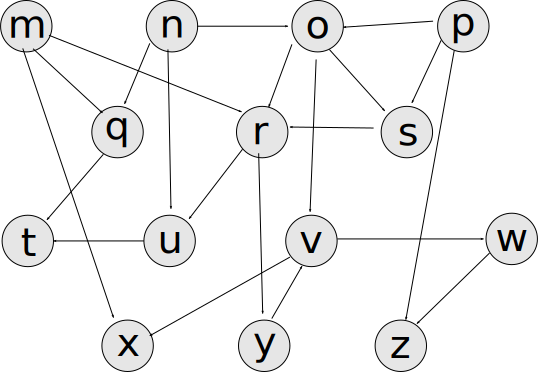
\includegraphics[width=120pt]{hw5-fig-22-8.pdf}
\end{center}
\answer
Denote the number of paths from $s$ to $u$ by $P(s, u)$, we calculate it recursively by
\begin{equation*}
P(s, u)=\left\{\begin{array}{ll}
\sum_{w \leadsto u}P(s, w)& (u \neq s)\\
0 & (u = s)\\
\end{array}\right.
\end{equation*}
Note that if a vertex $u$ does not have a parent, then $\sum_{w\leadsto u}P(s, w) = 0$, since there are no such parent $w$ vertices. And since the input is directed acyclic
graph, the recursion will terminate.

The algorithm is given below, an array $P$ is used to cache caculated results. $P$ is empty when calling for the first time.

\begin{algorithm}[H]
\caption{\textsc{Path-Count}$(G, P, s, t)$}
\If{$s = t$}{
  \Return $1$\\
}\Else{
  $S \leftarrow 0$\\
  \ForEach{parent vertex $w$ of $t$}{
    \If{$P[w]$ = nil} {
      $P[w]\leftarrow $\textsc{Path-Count}$(G, P, s, w)$
    }
    $S\leftarrow S + P(w)$
  }
  \Return $S$
}
\end{algorithm}

Line $4 \& 7$ is executed $O(V)$ times; line $6\&8$ is executed $O(E)$ times, since every edge will be checked only once when finding parent vertices. Thus we know the overall running time will be $O(V + E)$.
\qed

\problem{22.5-7}
A directed graph $G=(V, E)$ is said to be \textbf{\textsl{semiconnected}} if, for all pairs of vertices $u, v\in V$, we have $u\leadsto v$ or $v\leadsto u$. Give an efficient algorithm
to determine whether or not $G$ is semiconnected. Prove that your algorithm is correct, and analyze its running time.

\answer
First of all, we give the algorithm:

\begin{algorithm}[H]
\caption{\textsc{Is-Semiconnected}$(G)$}
$G' \leftarrow $\textsc{Strongly-Connected-Components}$(G)$\\
\If {$|V(G')|=1$}{
  \Return True
}\Else {
  $L \leftarrow$\textsc{Topological-Sort}$(G')$\\
  \For{$i = 1$ to $length[L]-1$}{
    \If{$(L[i], L[i + 1]) \notin E(G')$}{
      \Return False
    }
  }
  \Return True
}
\end{algorithm}

Now we explain how it works. It is trivial that strongly connected components are \textbf{\textsl{semiconnected}}, so first we shrink the original graph $G$ into $G'$ by finding
its strongly connected components. If $G'$ has only one vertex, it means the whole graph $G$ is strongly connected and thus \textbf{\textsl{semiconnected}}.
Otherwise, we run \textsc{Topological-Sort} on graph $G'$, line up its nodes in a list $L$. And then we check if any consecutive pair of vertices in $L$ is connected by an edge in $G'$.
If it is true, then for any $s, t\in G$, we can find corresponding $s', t'\in G'$ (and suppose $s'\neq t'$, in which case they are in the same strongly connected
components, and is discussed above), and either $s' \rightarrow L[i]\rightarrow L[i + 1] \rightarrow \cdots \rightarrow t'$
or $t' \rightarrow L[j] \rightarrow L[j + 1] \rightarrow \cdots \rightarrow s'$ in $L$. Thus we claim the graph $G$ is \textbf{\textsl{semiconnected}}.

Now we prove the algorithm is correct. According to the explanation above, \textsc{Is-Semiconnected} returns true only when the graph is \textbf{\textsl{semiconnected}}.
Suppose \textsc{Is-Semiconnected} returns false, which only happens when there is $(L[k], L[k + 1])\notin E(G')$. Since $L$ is a topological sort of $G'$, it is impossible
that $L[k + 1] \leadsto L[k]$. Now we have proved that neither $L[k] \leadsto L[k + 1]$ nor $L[k + 1] \leadsto L[k]$. So by choosing $s, v\in G$ corresponding to $L[k], L[k +1]\in G'$,
the graph $G$ cannot be \textbf{\textsl{semiconnected}}. Thus \textsc{Is-Semiconnected} returns false only when the graph is not \textbf{\textsl{semiconnected}}.

Finally, since both \textsc{Strongly-Connected-Components} \& \textsc{Topological-Sort} could be done in $O(V + E)$, and line $7$ is executed $O(V)$ times (at most $V$ items in $L$),
we know that \textsc{Is-Semiconnected} runs in $O(V + E)$.
\qed


\problem{22-2 Articulation points, bridges, and biconnected components}
Let $G=(V, E)$ be a connected, undirected graph. An \textbf{\textsl{articulation point}} of $G$ is a vertex whose removal disconnects $G$. A \textbf{\textsl{bridge}} of $G$ is an edge
whose removal disconnects $G$. A \textbf{\textsl{biconnected component}} of $G$ is a maximal set of edges such that any two edges in the set lie on a common simple cycle. The following figure
illustrates these definitions. We can determine articulation points, bridges, and biconnected components using depth-first search. Let $G_{\pi} = (V, E_\pi)$ be a depth-first tree of
$G$.

\begin{center}
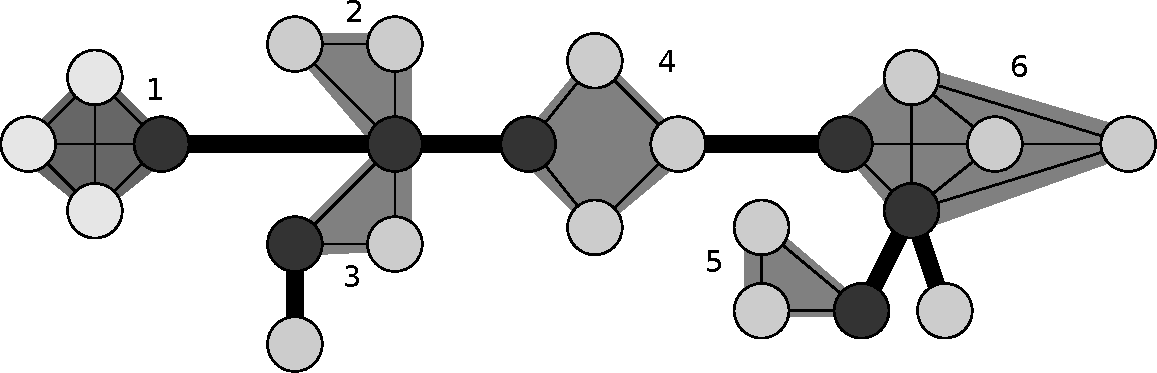
\includegraphics[width=300pt]{hw5-fig-22-10.pdf}
\end{center}

{
\small{
The articulation points, bridges and biconnected components of a connected, undirected graph for use in this problem. The articulation points are the heavily shaded vertices, teh bridges
are the heavily shaded edges, and the biconnected components are the edges in the shaded regions, with a $bcc$ number shown.}
}

\begin{description}
\item[a. \hspace{9pt}] Prove that the root of $G_\pi$ is an articulation point of $G$ if and only if it has at least two children in $G_\pi$.

\item[b. \hspace{9pt}] Let $v$ be a nonroot vertex of $G_\pi$. Prove that $v$ is an articulation point of $G$ if and only if $v$ has a child $s$ such that there is no back edge from $s$ or
any descendant of $s$ to a proper ancestor of $v$.

\item[c. \hspace{9pt}] Let
\begin{equation*}
low[v] = \min\left\{
  \begin{array}{l}
    d[v],\\
    d[w]:(u, w)\text{is a back edge for some descendent $u$ of $v$.}
  \end{array}
\right.
\end{equation*}

Show how to compute $low[v]$ for all vertices $v\in V$ in $O(E)$ time.

\item[d. \hspace{9pt}] Show how to compute all articulation points in $O(E)$ time.

\item[e. \hspace{9pt}] Prove that an edge of $G$ is a bridge if and only if it does not lie on any simple cycle of $G$.

\item[f. \hspace{9pt}] Show how to comput all the bridges of $G$ in $O(E)$ time.

\item[g. \hspace{9pt}] Prove that the biconnected components of $G$ partition the nonbridge edges of $G$.

\item[h. \hspace{9pt}] Give an $O(E)$-time algorithm to label each edge $e$ of $G$ with a positive integer $bcc[e]$ such that $bcc[e] = bcc[e']$ if and only if $e$ and $e'$ are
in the same biconnected component.

\end{description}
\answer

\begin{description}

\item[a. \hspace{9pt}] 

\textbf{root of $G_\pi$ is articulation point $\Rightarrow$ it has at least two children in $G_\pi$ :}

We prove by contradiction. Label the root point as $V_{root}$, and suppose it has less than 2 children in $G_\pi$. If $V_{root}$ has no children, then $V_{root}$ is the only
vertex in $G_pi$, and it is trivial that $V_{root}$ cannot be an articulation point. If $V_{root}$ has only one children $V_1$, then cutting $V_{root}$ off in  $G$ will still
left the subtree with root at $V_1$ connected, thus $V_{root}$ cannot be an articulation point. So $V_{root}$ must has at least 2 children in $G_\pi$. \\

\textbf{root of $G_\pi$ has at least two children in $G_\pi$ $\Rightarrow$ it is articulation point :}

Choose 2 children of $V_{root}$, label them as $V_1, V_2$, and the corresponding subtrees as $T_1, T_2$. First of all, there cannot be vertices $u\in T_1, v\in T_2$ such that $(u, v)\in E$,
otherwise according to DFS algorithm, $u, v$ should be in the same subtree, which is a contradiction to the fact that  $T_1 \cap T_2=\emptyset$. So by cutting $V_{root}$ off, subtree $T_1$ and $T_2$
will be disconnected, which means $V_{root}$ is an articulation point.

\item[b. \hspace{9pt}]

\textbf{``if'' side :}
% got this from pdfqueen
Assume that $v$ is an articulation point of $G$. Let $C_r$ be the connected component of $G-v$ containing the root of the tree $G_{\pi}$. Let $s$ be a neighbor of $v$ that is not in $C_r$
(this neighbor must exist since removing $v$ must create at least two connected components) and $C_s$ be the connected component containing $s$. In $G_\pi$, all the proper ancestors of
$v$ are in $C_r$, and all the descendants of $s$ are in $C_s$. Thus, there can be no edges between descendants of $s$ and proper ancestors of $v$.

\textbf{``only if'' side :}

Label the subtree at $v$ as $T_v$, and subtree at $s$ as $T_s$. By DFS algorithm, it is trivial that no vertex in $T_s$ could be connected to its sibling subtrees, so is true with $T_v$.
So we know that no vertex in $T_s$ could be connected to sibling trees of $T_s$, or $T_v$. And since no vertex in $T_s$ is connected to a proper ancestor of $v$, we know that by cutting
$v$ off, the whole subtree $T_s$ is disconected from other part of the graph. So $v$ is an articulation point.

\item[c. \hspace{9pt}]
% got this from pdfqueen
 
We can compute $low[v]$ for all vertices $v$ by starting at the leaves of the tree $G_\pi$. We compute $low[v]$ as follows:

$$low[v] = \min\left(d[v], \min_{y\in children(v)}low[y], \min_{backedge(v, w)}d[w]\right).$$

For leaves $v$, there are no descendants $u$ of $v$, so this returns either $d[v]$ or $d[w]$ if there is a back edge $(v, w)$. For vertices $v$ in the tree, if $low[v] = d[w]$, then either
there is a back edge $(v, w)$, or there is a back edge for some descendant $u$. The last term in the $\min$ expression handles the case where $(v, w)$ is a back edge. If $u$ is a descendant of
$v$ in $G_\pi$, we know that $d[u] > d[v]$ since $u$ is visited after $v$ in the DFS. Therefore, if $d[w] < d[v]$, we also have $d[w]< d[u]$, so we will have $low[u] = d[w]$. The middle term
in the $\min$ expression therefore handles the cases where $(u, w)$ is a back edge for some descendant $u$. Since we start at the leaves of the tree and work our way up, we will have computed
everything we need when computing $low[v]$.

For each node $v$, we look at $d[v]$ and something related to all the edges leading from $v$, either tree edges leading to the children or back edges. So, the total running time is linear in
the number of edges in $G$, i.e., $O(E)$.

\item[d. \hspace{9pt}] From (c) we could infer that $low[v] \leq d[v] \iff v$ is an articulation point. So we could find all the articulation points while calculating $low$ values.
Since calculation of $low$ value takes $O(E)$ time, finding articulation points will also take $O(E)$ time.

\item[e. \hspace{9pt}]

\textbf{``if'' side :}

Label the edge as $e^* = (u, v)$. We prove by contradiction. Suppose $e^*$ lies on a simple cycle $u - v - w_1 - w_2 - \cdots w_k - u$ of $G$. Consider 2 vertices $x, y$ which
is connected by path $x-x_1 -\cdots x_i - u - v - y_1 - y_2 \cdots y_j - y$. When $e^*$ is removed, $x, y$ is still connected by path $x - x_1 - \cdots x_i - u - w_k - \cdots w_1 -v- y_1 -
\cdots y_j -y$. Thus removing $e^*$ will not change the connectivity of $G$, which is a contradiction. From this we have proved  the ``if'' side.

\textbf{``only if'' side :}
% got this from pdfqueen

We prove by contradiction. Assume $(u, v)$ is not on a simple cycle, and it is not a bridge. Now remove the edge $(u, v)$. Since $(u, v)$ is not a bridge, there is still another path
connecting $u$ and $v$, say $u -x_1 -\cdots -x_i - v$. Then, the edges $u - v - x_i -\cdots-x_1 - u$ is a cycle, which is a contradiction. So $(u, v)$ must be a bridge.

\item[f. \hspace{9pt}] 
% got this from pdfqueen

Any bridge in the graph $G$ must exist in the graph $G_\pi$. Otherwise, assume $(u, v)$ is a bridge and that we explore $u$ first. Since removing $(u, v)$ disconnects $G$, the only way to
explore $v$ is through the edge $(u, v)$. So, we only need to consider the edges in $G_\pi$ as bridges. If there are no simple cycles in the graph that contains the edge $(u, v)$ and we
explore $u$ first, then we know that there are no back edges between $v$ and anything else. Also, we know that anything in the subtree of $v$ can only have back edges to other nodes in 
the subtree of $v$. Therefore, we will have $low[v] = d[v]$ since $v$ is the first node visited in the subtree rooted at $v$. Thus, we can look over all the edges of $G_\pi$ and see
whether $low[v] = d[v]$. If so, then we will output that $(parent[v]_{g_\pi}, v)$ is a bridge, i.e. that $v$ and its parent in $G_\pi$ form a bridge. Computing $low[v]$ for all vertices
$v$ takes time $O(E)$ as we showed in (c). Looping over all the edges takes time $O(V)$ since there are $(V-1)$ edges in $G_\pi$. Thus the total time to calculate the bridges in $G$ is
$O(E)$.

\item[g. \hspace{9pt}]
% got this from pdfqueen

Since \textbf{an edge is a bridge of $G \iff$  it is not on any simple cycle of $G$}, it is equivalent to the fact that \textbf{an edge is a nonbridge edge $\iff$ it is on any simple cycle of $G$}. Since
\textbf{an edge is in the biconnected component $\iff$ it is on any simple cycle of $G$}, we get the fact that \textbf{if the edge is in the biconnected components of $G \iff $ it is a nonbridge edge}.
Thus, the biconnected components partition the nonbridge edges of $G$.

\item[h. \hspace{9pt}]

The biconnected components are disconnected to each other by bridges and articulation points. First of all, we use $O(E)$ time to find out all the articulation points, and bridges.
Then cut off all bridges from $G$, and run DFS on $G$. Note that when performing DFS, if we visited an articulation point, mark it with green color, and checks if it has green colored
neighbors (also articulation points). If it has such a neighbor, add the edge in to DFS tree, otherwise stop running DFS on this articulation point. When the DFS finished, give edges in
different DFS trees with different $bcc$ value. There are $O(E)$ edges to check, so the DFS phase takes $O(E)$ time, thus the overall time is $O(E)$.
\end{description}
\qed

\problem{22-4 Reachability}
Let $G=(V, E)$ be a directed graph in which each vertex $u\in V$ is labeled with a unique integer $L(u)$ from the set $\{1, 2, \ldots, |V|\}$. For each vertex $u\in V$, let
$R(u) = \{v\in V: u\leadsto v\}$ be the set of vertices that are reachable from $u$. Define $\min(u)$ to be the vertex in $R(u)$ whose label is minimum, i.e., $\min(u)$ is
the vertex $v$ such that $L(v) = \min\{L(w):w\in R(u)\}$. Give an $O(V + E)$-time algorithm that computes $\min(u)$ for all vertices $u\in V$.

\answer
For any $u, v$ in the same strongly connected component, we have $R(v)=R(u)$ (if $v \leadsto w$, then $u \leadsto v \leadsto w$, vice vesa), thus $\min(v)=\min(u)$. So we could
shrink the original graph to $G'$ by finding its strongly connected components. Define $\min^*(u)$, which is identical to $\min(u)$ except that it only considers vertices in
the strongly connected component $S$ ($u \in S$).
Let $v^*\in S$ be the vertex such that $L(v^*) = \min\{L(w):w\in S\}$, then we have
$$\min_{u\in S}^*(u) = v^*.$$

Then, by running topological sort on the shrinked graph $G'$, we get list of nodes $L$. We could then calculate $\min$ value from $\min^*$ value, from the last element in $L$ back
to the first element in $L$ using the following:
$$\min(u) = \left\{\begin{array}{ll}
\min_{v : u \leadsto v}\{\min(v)\} & (u \text{ has children vertices})\\
\min^*(u) & (u \text{ does not have children vertices})
\end{array}\right.
$$

The algorithm is given below. Since \textsc{Topology-Sort} and \textsc{Strongly-Connected-Components} runs in $O(V + E)$ time, and finally calculating $\min$ value from topology
sort result takes $O(E)$ time, the overall running time is $O(V + E)$.

\begin{algorithm}[H]
\caption{\textsc{Calculate-Reachability}$(G)$}
Initialize hash table $M$\tcp*[r]{$M$ is used to store $\min$ value}
Initialize hash table $M'$\tcp*[r]{$M'$ is used to store $\min^*$ value}
$G' \leftarrow $\textsc{Strongly-Connected-Components}$(G)$\\
\ForEach{strongly connected component $S$ in $G$}{
  Denote $u\in G'$ as the vertex corresponding to $S$\\
  $M'[u] = \min_{v}\{L(v): v\in S\}$\tcp*[r]{calculate $\min^*$ value}
}
$\Gamma \leftarrow $\textsc{Topology-Sort}$(G')$\\
\For{$i = length[\Gamma]$ \text{\textnormal{\textbf{downto}}} $1$}{
  \If{$\Gamma[i]$ has children vertices}{
    $M[i] = \min_{v: v\leadsto \Gamma[i]}\{M[v]\}$
  }\Else{
    $M[i] = M'[i]$
  }
}
\Return $M$
\end{algorithm}
\qed




\chapter{Homework 6}
\problem{15.1-1}
Show how to modify the \textsc{Print-Stations} procedure to print out the stations in increasing order of station number.
\answer

The algorithm is given below:

\begin{algorithm}[H]
\caption{\textsc{Print-Stations-New}$(l, n)$}
\textsc{Print-Stations-Recursive}$(l, l^*, n)$
\end{algorithm}

\begin{algorithm}[H]
\caption{\textsc{Print-Stations-Recursive}$(l, i, j)$}
\If{$j \neq 1$}{
  \textsc{Print-Stations-Recursive}$(l, l_i[j], j - 1)$\\
}
\textbf{Print} ``line '' $i$ ``, station '' $j$
\end{algorithm}
\qed

\problem{15.1-2}
Use the following equations and the substitution method to show that $r_i(j)$, the number of references made to $f_i[j]$ in a recursive algorithm, equals $2^{n-j}$.
\begin{eqnarray*}
r_1(n)&=& r_2(n) = 1,\\
r_1(j) &=& r_2(j) = r_1(j + 1) + r_2(j + 1).
\end{eqnarray*}
\answer
For the case of $j = n$, we have $r_i(j) = 1 (= 2^{n - j})$. Suppose when $j = n_0$, we have $r_i(j) = 2^{n - j}(=2^{n-n_0})$, then for the case of $j = n_0 - 1$, we have:

\begin{eqnarray*}
r_i(j) &=& r_1(j + 1) + r_2(j + 1)\\
&=& r_1(n_0) + r_2(n_0)\\
&=& 2^{n - n_0} + 2^{n - n_0}\\
&=& 2^{n - (n_0 + 1)}.
\end{eqnarray*}

So by mathematical induction we know that $r_i(j) = 2^{n - j}$.
\qed

\problem{15.2-1}
Find and optimal parenthesization of a matrix-chain product whose sequence of dimensions is $\langle5, 10, 3, 12, 5, 50, 6\rangle$.
\answer
\todo
\qed


\problem{15.2-2}
Give a recursive algorithm \textsc{Matrix-Chain-Multiply}$(A, s, i, j)$ that actually performs the optimal matrix-chain multiplication, given the sequence of matrices 
$\langle A_1, A_2, \ldots, A_n\rangle$, the $s$ table computed by \textsc{Matrix-Chain-Order}, and the indices $i$ and $j$. The initial call would be \textsc{Matrix-Chain-Multiply}$(A, s, 1, n)$.
\answer
\todo
\qed


\problem{15.3-3}
Consider a variant of the matrix-chain multiplication problem in which the goal is to parenthesize the sequence of matrices so as to maximize, rather than minimize, the number of
scalar multiplications. Does this problem exhibit optimal substructure?
\answer
\todo
\qed

\problem{15.3-4}
Describe how assembly-line scheduling has overlapping subproblems.
\answer
\todo
\qed

\problem{15.4-5}
Give an $O(n^2)$-time algorithm to find the longest monotonically increasing subsequence of a sequence of $n$ numbers.
\answer
\todo
\qed

\problem{15.5-2}
Determine the cost and structure of an optimal binary search tree for a set of $n=7$ keys with the following probabilities:
\begin{center}
\begin{tabular}{|c|cccccccc|}
\hline
$i$ & 0 & 1 & 2 & 3 & 4 & 5 & 6 & 7\\
\hline
$p_i$ & & 0.04 & 0.06 & 0.08 & 0.02 & 0.10 & 0.12 & 0.14\\
$q_i$ & 0.06 & 0.06 & 0.06 & 0.06 & 0.05 & 0.05 & 0.05 & 0.05\\
\hline
\end{tabular}
\end{center}
\answer
\todo
\qed

\problem{25.1-4}
Show that matrix multiplication defined by \textsc{Extend-Shortest-Paths} is associative.
\answer
\todo
\qed

\problem{25.2-4}
The \textsc{Floyd-Warshall} algorithm requires $\Theta(n^3)$ space, since we need to compute $d_{ij}^{(k)}$ for $i, j, k = 1, 2, \ldots, n$. Show that the following
procedure, which simply drops all the superscripts, is correct, and thus only $\Theta(n^2)$ space is required.

\begin{algorithm}[H]
\caption{\textsc{Floyd-Warshall'}$(W)$}
$n \leftarrow rows[W]$\\
$D \leftarrow W$\\
\For{$k \leftarrow 1$ \KwTo $n$} {
  \For{$i \leftarrow 1$ \KwTo $n$} {
    \For{$j \leftarrow 1$ \KwTo $n$} {
      $d_{ij}\leftarrow \min(d_{ij}, d_{ik} + d_{kj})$
    }
  }
}
\Return $D$
\end{algorithm}
\answer
\todo
\qed

\problem{25.2-6}
How can the output of the \textsc{Floyd-Warshall} algorithm be used to detect the presence of a negative-weight cycle?
\answer
\todo
\qed




\end{document}

